% REVIEW - Verificar palavras estrangeiras e siglas
\chapter[Fundamentação Teórica]{Fundamentação Teórica}
\addcontentsline{toc}{chapter}{Fundamentação Teórica}

A fundamentação teórica tem como objetivo apresentar os principais conceitos e tecnologias que embasam o desenvolvimento deste trabalho. São abordados temas como assistentes virtuais, sistemas de mensageria, automação de atendimento, bases de conhecimento e ferramentas utilizadas no projeto, bem como aspectos relacionados à organização institucional na universidade de brasília.

\section{Organização Institucional da UnB}

A Universidade de Brasília (UnB) é uma instituição federal de ensino superior localizada na capital do país, fundada em 1962, apenas dois anos após a inauguração de Brasília. Atualmente, a universidade conta com quatro campi: o principal, situado no Plano Piloto (Campus Darcy Ribeiro), e três localizados em regiões administrativas do Distrito Federal — Ceilândia, Gama e Planaltina. Juntas, essas unidades oferecem um total de 76 cursos de graduação, atendendo a uma comunidade acadêmica ampla e diversa. 

A UnB possui uma estrutura organizacional formalizada, conforme o organograma \cite{organogramaUnB2017}. No topo dessa estrutura está o Conselho Universitário (CONSUNI), órgão máximo deliberativo responsável por decisões estratégicas, tais como criação e extinção de cursos, aprovação do Regimento Geral e dos regimentos internos de Unidades Acadêmicas, Órgãos Complementares e Centros.

Abaixo do CONSUNI encontra-se a Reitoria, conduzida pelo Reitor, com o apoio da Vice‑Reitoria, responsáveis pela administração executiva da instituição, coordenando também os diversos decanatos, que cuidam das áreas de planejamento, extensão, pesquisa, administração e outras funções institucionais.

Posteriormente, encontram-se as unidades acadêmicas, compostas por institutos e faculdades, cada um subdividido em departamentos que organizam o ensino, a pesquisa, e as atividades de extensão em áreas específicas do conhecimento. Essas unidades têm autonomia para elaborar normativas internas, complementares às diretrizes gerais definidas em nível central.

Dessa forma, parte das normas institucionais são centralizadas, como políticas de matrícula, calendário acadêmico e procedimentos gerais, enquanto outras variam conforme a unidade acadêmica, como regras para estágios, validações curriculares e trâmites de colação de grau. Essas informações, embora públicas, costumam estar dispersas em editais, resoluções e manuais administrativos, geralmente em formato PDF, e organizadas por cada instância responsável.

\section{Chatbots}

Chatbots são programas de software desenvolvidos para simular interações humanas, seja por meio de texto ou voz, permitindo que usuários se comuniquem com sistemas computacionais como se estivessem conversando com uma pessoa real \cite{rouse2018chatbot,aws2025chatbot}. Esses agentes conversacionais podem ser incorporados em sites, aplicativos móveis, plataformas de mensagens instantâneas e assistentes virtuais, automatizando o atendimento ao usuário e facilitando o acesso à informação.

No cenário atual, os chatbots são classificados em dois grandes grupos, de acordo com sua complexidade e função \cite{oracle2025chatbot}:

\begin{itemize}
    \item \textbf{Chatbots orientados a tarefas (declarativos)}: são agentes com funções bem definidas e limitadas, geralmente baseados em regras fixas e processamento básico de linguagem natural (NLP). Eles são projetados para responder perguntas frequentes, agendar compromissos, realizar consultas simples e executar comandos específicos de forma estruturada. São os tipos mais comuns atualmente, especialmente em contextos de atendimento institucional e suporte técnico.
    % REVIEW - sigla sem definição
    \item \textbf{Chatbots orientados por dados (conversacionais ou preditivos)}: são sistemas mais avançados que utilizam tecnologias de inteligência artificial, aprendizado de máquina (ML), NLP e entendimento de linguagem natural (NLU) para compreender melhor as intenções do usuário, aprender com interações anteriores e oferecer respostas personalizadas. Esses chatbots são capazes de manter o contexto de uma conversa, prever necessidades e executar tarefas complexas com múltiplas variáveis. Exemplos desse tipo incluem assistentes como Siri (Apple) e Alexa (Amazon).
\end{itemize}

Em ambientes educacionais, a adoção de chatbots tem crescido significativamente, especialmente como ferramenta para fornecer informações institucionais, esclarecer dúvidas acadêmicas e facilitar a comunicação entre estudantes e setores administrativos. Seu uso contribui para tornar o ambiente universitário mais acessível, automatizando respostas e simplificando o acesso a informações relevantes de maneira contínua, imediata e personalizada \cite{dykeland2018unleashing}.

\section{Aplicações de Bots em Ambientes Educacionais}

A presença de assistentes virtuais no meio educacional tem se expandido rapidamente, impulsionada pelas vantagens em automatizar tarefas, ampliar o acesso à informação e oferecer suporte personalizado aos estudantes. Chatbots vêm sendo aplicados com sucesso em contextos diversos da educação superior, tanto para apoiar o aprendizado quanto para auxiliar em processos administrativos. Esses sistemas permitem aos estudantes interagirem com serviços da instituição de forma ágil, por meio de plataformas conhecidas como WhatsApp, Telegram ou Messenger.

% No trabalho de \textcite{hien2018fitebot}, destaca-se o desenvolvimento do FIT-EBot, um chatbot criado para atender demandas administrativas e acadêmicas dos estudantes de uma universidade vietnamita. O sistema foi treinado com base em dados institucionais e estruturado para responder perguntas frequentes sobre cronogramas, requisitos de disciplinas, notas, estágios, bolsas, entre outros. A avaliação feita com estudantes revelou um alto interesse na adoção do assistente virtual, especialmente pela facilidade de acesso e disponibilidade constante do serviço.

Tal experiência demonstra que o uso de chatbot em ambientes acadêmicos oferece benefícios concretos na comunicação, na eficiência dos atendimentos e na personalização das interações com os estudantes. Nesse sentido, a proposta deste trabalho, desenvolver um assistente virtual voltado ao suporte institucional para alunos da Universidade de Brasília, mostra-se coerente com tendências consolidadas e encontra respaldo na literatura recente. A ferramenta buscada poderá reunir, estruturar e facilitar o acesso a informações normativas e administrativas.

\section{Sistemas de Mensageria: WhatsApp e Telegram}

A popularização dos aplicativos de mensagens instantâneas transformou significativamente as formas de comunicação interpessoal e institucional. No contexto acadêmico, essas plataformas tornaram-se canais estratégicos para a troca de informações entre estudantes, professores e setores administrativos. Dentre os aplicativos disponíveis, destacam-se o WhatsApp e o Telegram, amplamente utilizados pela população brasileira.

Considerando seu amplo alcance, praticidade e familiaridade entre os usuários, esses sistemas de mensageria têm sido cada vez mais explorados como interfaces para soluções automatizadas de atendimento, como é o caso dos chatbots institucionais. A escolha dessas plataformas como meio de entrega de informações acadêmicas torna-se, portanto, não apenas viável, mas também estratégica, ao alinhar a tecnologia à realidade cotidiana dos estudantes.

Segundo dados da pesquisa Panorama Mobile Time/Opinion Box (2024), o WhatsApp mantém-se como o aplicativo de mensageria mais presente nos smartphones brasileiros, instalado em 98\% dos dispositivos. O Telegram, por sua vez, apresentou crescimento significativo nos últimos anos, saltando de 13\% de presença em janeiro de 2019 para um pico de 66\% em agosto de 2023, com leve recuo para 63\% em janeiro de 2024.

% \begin{figure}[h]
% 	\centering
% 	\label{fig01}
% 		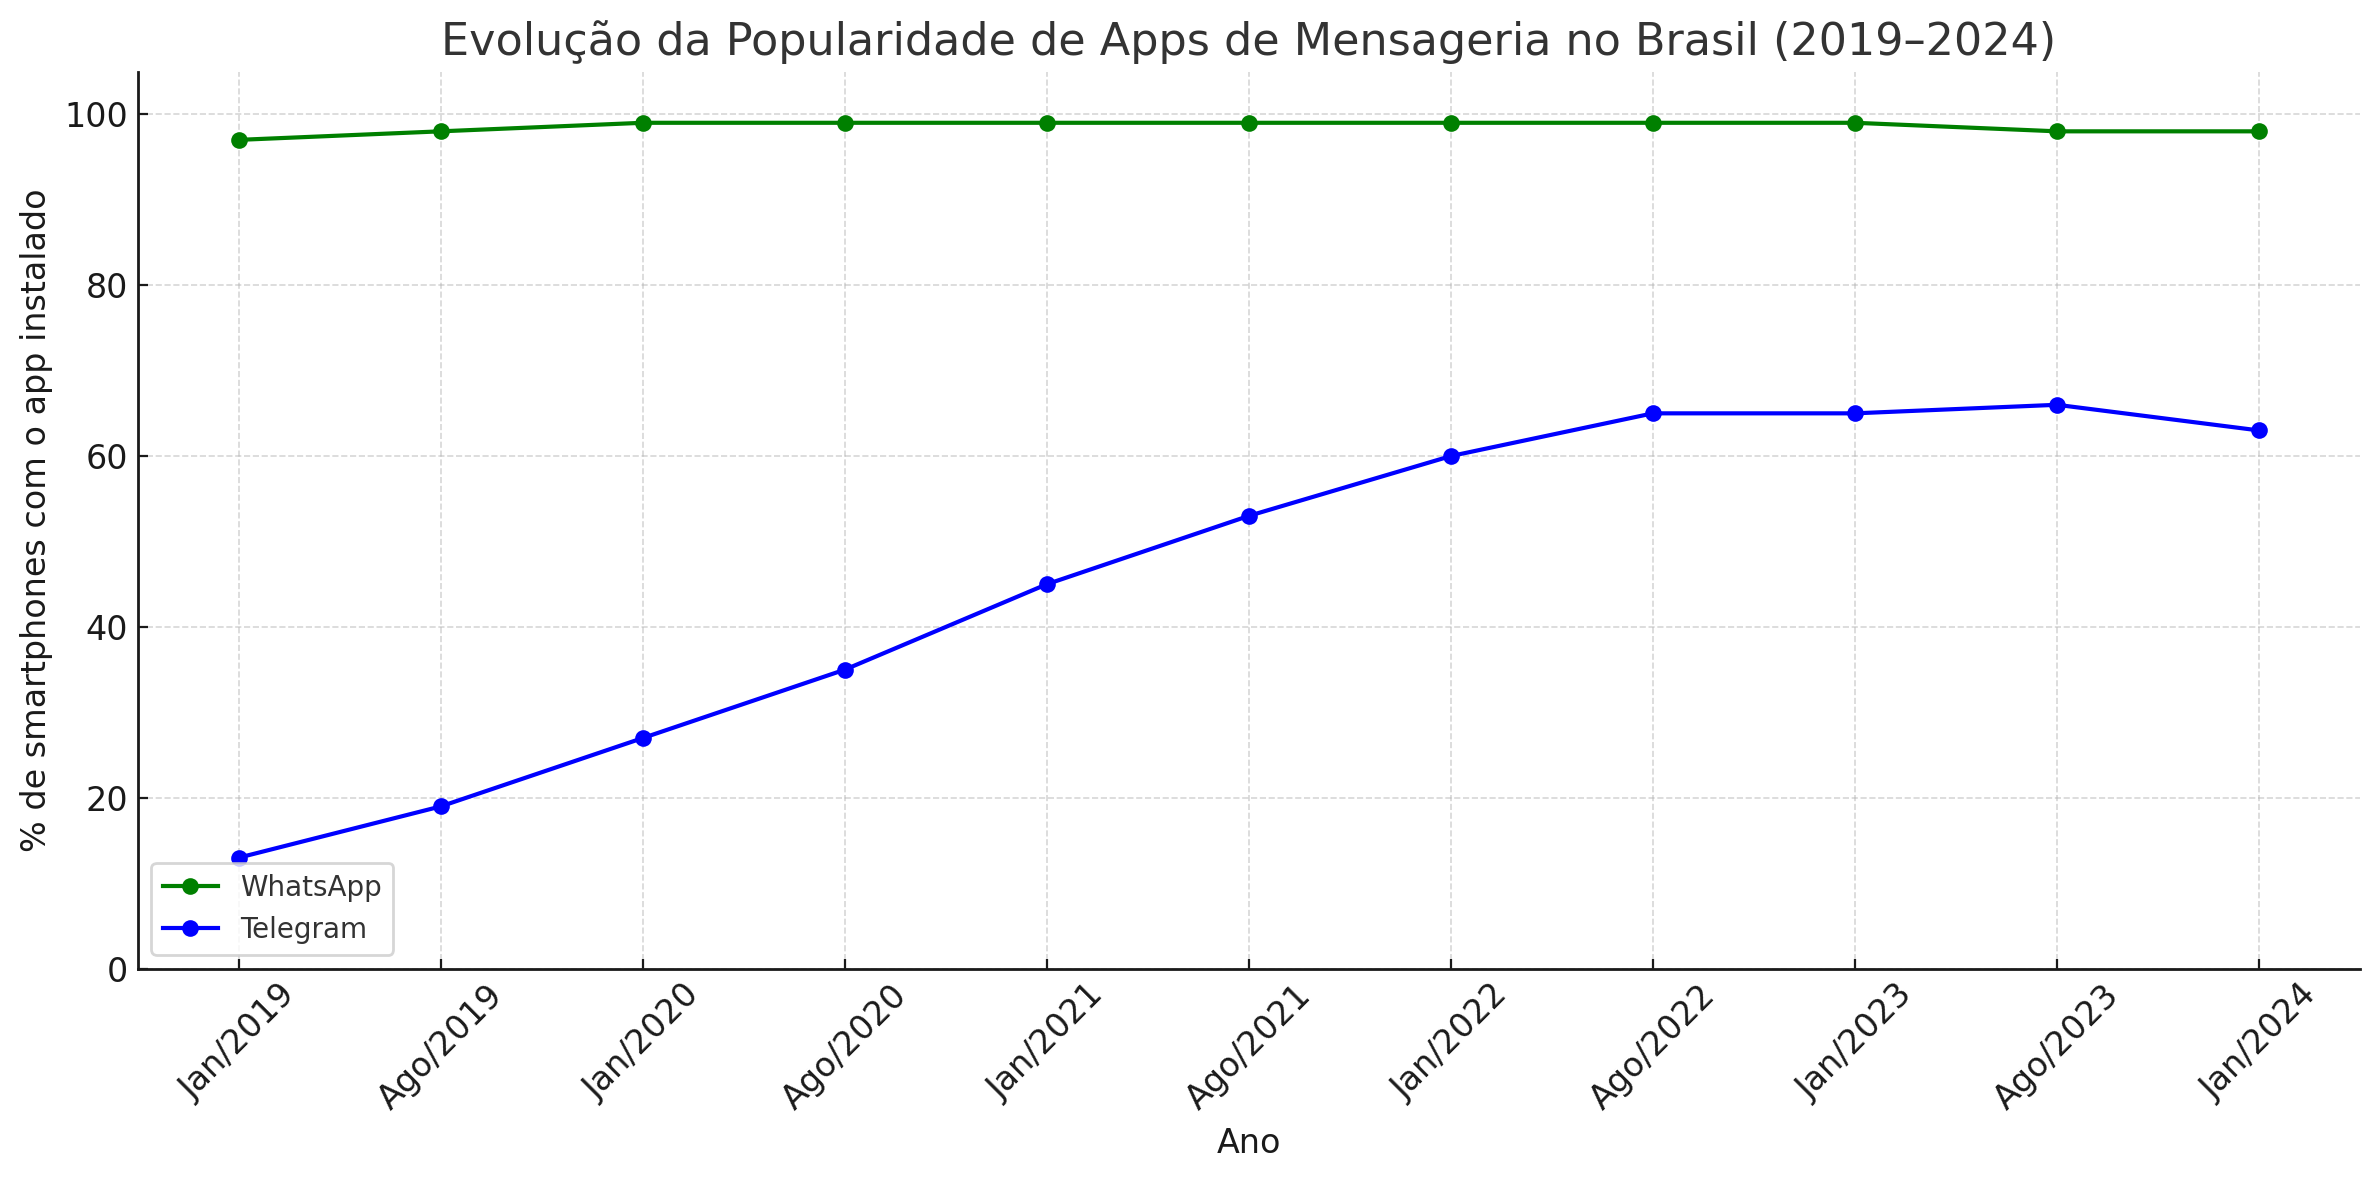
\includegraphics[keepaspectratio=true,scale=0.3]{figuras/grafico-mensageiros.png}
% 	\caption{Evolução da popularidade de WhatsApp e Telegram no Brasil (2019–2024). Fonte: Panorama Mobile Time/Opinion Box, 2024.}
% \end{figure}

Diante da expressiva presença dessas plataformas entre os usuários brasileiros, especialmente no contexto universitário, evidencia-se que tanto o WhatsApp quanto o Telegram são canais altamente relevantes para o desenvolvimento de soluções automatizadas de suporte institucional. O alcance praticamente universal do WhatsApp, aliado ao crescimento contínuo do Telegram, reforça o potencial dessas ferramentas para garantir acessibilidade, engajamento e efetividade na comunicação com os estudantes. Considerando ainda os resultados da pesquisa realizada com alunos da Universidade de Brasília, torna-se estratégica a escolha dessas plataformas como meios de interação para o assistente virtual proposto, visando atingir o maior número possível de estudantes e facilitar o acesso a informações institucionais.

\section{Tecnologias e Ferramentas Utilizadas}

O desenvolvimento do assistente virtual proposto será realizado com base em tecnologias modernas e acessíveis. Dentre as ferramentas e linguagens consideradas, destacam-se:

\begin{itemize}
    \item \textbf{Python}: Linguagem de programação utilizada para o desenvolvimento do bot e do backend.
    \item \textbf{Flask / FastAPI}: Frameworks web leves e ideais para APIs e microserviços.
    \item \textbf{MongoDB ou SQLite}: Banco de dados para armazenamento da base de conhecimento.
    \item \textbf{Telegram Bot API}: Plataforma principal para teste e validação do protótipo.
\end{itemize}

O uso dessas tecnologias visa garantir baixo custo de desenvolvimento, facilidade de manutenção e rápida implantação em ambiente universitário.
